% Chapter 2 - Infraestructura

\chapter{Infraestructura} % Chapter title

\label{ch:infra} 

%----------------------------------------------------------------------------------------

% ### Introducción de capitulo

En los trabajos analizados en el capitulo \ref{ch:estado_arte}, las soluciones propuestas han necesitado algún conjunto mínimo de capas de abstracción, que les permita brindar el soporte para la conexión o el agregado de alguna modalidad especifica en un sistema particular.

El trabajo de \citet{dumas2009multimodal} presenta una arquitectura genérica para el desarrollo de aplicaciones multimodales, como se puede ver en la figura \ref{fig:arq_others_dumas}. Esta será una referencia importante en esta parte del documento.

En el presente capitulo se introducirán las decisiones de bajo nivel de la solución propuesta para la conexión de nuevas modalidades al contexto de una aplicación web, las mismas constituirán la plataforma denominada \emph{Plusultra}. 

Primero se describen las características generales de las aplicaciones web (clientes de la plataforma), para luego introducir las decisiones arquitectónicas. En el siguiente capitulo se completan los aspectos de desarrollo, añadiendo el modulo cliente (que corre en las aplicaciones web).
%Aquí se mostrará la estrategia seleccionada para desarrollar la plataforma.

\section{Características de las Aplicaciones Web} \label{sec:web_app_def}

El concepto de \emph{aplicación web} ha evolucionado desde sus inicios, con algunos pasos destacados como el surgimiento de AJAX en los 90s, que introdujo una nueva capa en el cliente mediante un conjunto de tecnologías con el fin de fragmentar la comunicación con el servidor, mejorando la experiencia de usuario; según indica \citet{garrett2005ajax}. Desde ese momento, las aplicaciones web fueron delegando, consistentemente, lógica de negocio hacia el cliente. 

En los últimos años, han surgido conceptos desde el ámbito académico como RIA (Rich Internet Applications) \citep{Fraternali2010}, que busca dar un marco conceptual a dicho movimiento. Por el lado de la industria, el desplazamiento hacia el cliente también es claro, librerías como Backbone.js \citep{ind:backbone} (desde el 2010), como una de las mas populares e inspiradoras para otros frameworks como Ember.js \citep{ind:ember} y Angular.js \citep{ind:angular}, han llevado el paradigma MVC fuera del servidor.

Por otra parte, el proyecto Node.js \citep{infra:nodejs}, a través de V8, permite la utilización de JavaScript del lado del servidor. Esta característica ha generado versatilidad en el software desarrollado, la misma puede observarse con proyectos como \emph{Browserify} \citep{infra:browserify} que posibilita la generación de módulos híbridos, capaces de correr en ambos extremos (cliente y servidor). Teniendo en cuenta esto, sumado a la ya conocida sólida presencia de JavaScript, como lenguaje estándar en el entorno del navegador, ha impulsado el ecosistema de desarrollo en JavaScript, posicionando a npm, como uno de los manejadores de paquetes mas populares hoy en día \citep{infra:npm-mods}. 

\subsection{Aspectos Particulares de las Aplicaciones Web Actuales}

Las aplicaciones web han evolucionado tomando formas similares a las de las aplicaciones de escritorio. Es decir, aplicaciones tipo single-page (SPA), con  múltiples componentes de interfaz de usuario que permitan la interacción con datos in-situ sin necesidad de refrescar o navegar a diferentes secciones.
Por \emph{single page applications} (SPA) o \emph{single page interface} (SPI)\citep{infra:spamanifesto} se hace referencia a aquellas aplicaciones web que cuentan con las siguientes características: minimizan la carga inicial de componentes a un request (\emph{single page load}), modularizan el contenido JavaScript (abstrayendo las llamadas AJAX con el servidor), tienen capacidad de manejar ruteo y la historia del navegador, soporte de templates \emph{client-side}, comunicación bidireccional (\emph{real-time}) con el servidor y capacidad de usar almacenamiento local en el cliente. 

El concepto de RIA (\emph{Rich Internet Applications}) define estos nuevos tipos de aplicaciones. Es decir, el cambio que hubo desde compartir contenido estático hasta el dinamismo actual.
Con el fin de expandir las características definidas a través del termino \emph{RIA} y buscando describir mas estrictamente el escenario donde serán incluidas la capacidad de usar múltiples modalidades, se define el siguiente listado de características que hacen a una aplicación web actual:

\begin{itemize}
\item \textbf{Aplicaciones inherentemente distribuidas}; de acuerdo al paradigma de comunicaciones cliente-servidor, aún vigente en la web, las aplicaciones se conectan al servidor para obtener algo y realizar alguna tarea, el servidor luego puede centralizar resultados. En la web, ocurre algo similar, las aplicaciones web, a través de los agentes de usuario, descargan toda la aplicación, incluso algún conjunto de datos básico; esto le permite al usuario interactuar con la aplicación en su completitud e incluso de forma ''offline'' si se adecuan algunos parámetros.

\item \textbf{Aplicaciones inherentemente multiplataforma}; luego del surgimiento de la \emph{web 2.0}, se consolida la web como plataforma (\emph{Web as a plataform}), este concepto se apoya en la multiplicidad de servicios que la web ofrece o que una aplicación desarrollada para este ecosistema puede consumir, de acuerdo a \citet{infra:html5}. Estos servicios, son ofrecidos a través de vínculos nativos, por el navegador del usuario. Las aplicaciones son codificadas en lenguajes estándares, que corren dentro del ambiente provisto por el navegador.

\item \textbf{Clientes ``pesados'' con características de aplicaciones de escritorio}; la lógica de aplicación ya no se encuentra totalmente en el servidor. El servidor provee funciones de centralización (\ie  autenticación) o recursos a través de \emph{APIs} (\ie  REST); pero la manipulación y el tratado de los mismos ocurre del lado del cliente.

\item \textbf{APIs estándar para consumo de características nativas de hardware}; a través de la W3C, se busca expandir la web en múltiples direcciones. En \citep{infra:html5} se listan varios de estos tópicos. Por ejemplo, se destaca, la API de Vibración \citep{infra:vibration} o la especificación para el acceso a eventos táctil \citep{infra:touch}; las mismas definen como utilizar diferentes capacidades de interacción.

\item \textbf{Adaptabilidad}; mediante estrategias como \emph{responsive-design} es posible no solo adaptar contenido de acuerdo a la pantalla del dispositivo, si no también, a las características disponibles de cada uno. Se desarrolla buscando una mejora progresiva. Entre otras ventajas, esto permite mantener una única base de código en lugar de diseñar diferentes aplicaciones, tanto para escritorio como para dispositivos móviles.

\marginpar{Socket.io y WS, son proyectos open source, desarrollados en JavaScript, que implementan el protocolo WebSocket. Si bien difieren en como lo implementan, ambas 
librerías permiten crear clientes y servidores de WebSockets.}

\item \textbf{Bidireccional en el inicio de la conversación}; \emph{Web Sockets} es otra especificación de la W3C \citep{infra:websockets}, con implementaciones concretas utilizadas por la industria, como \href{http://socket.io/}{Socket.io} o \href{http://einaros.github.io/ws/}{WS}, entre otras; permiten la comunicación bidireccional entre cliente y servidor y el ``inicio de la conversación'' por parte de las aplicaciones web. Esto posibilita un escenario con características de \emph{tiempo-real}.
\end{itemize}

\section{Arquitectura Propuesta} \label{sec:arq_ours}
Teniendo en cuenta el escenario planteado, insertar de forma genérica una nueva modalidad implica algunos desafíos técnicos. A continuación se describe la estrategia elegida y su fundamentación. La misma se compone, a grandes rasgos, de tres partes; dos \emph{APIs}, una para el navegador como una dependencia mas de la aplicación web y la otra para conectar la nueva modalidad al entorno web; el componente restante es una pasarela de mensajes. Es el componente que sera descrito en este capitulo, los otros dos serán tratados mas adelante.

% FIGURA DE COMPONENTES ARQ - single app
\begin{center}
  \begin{figure}[h]
    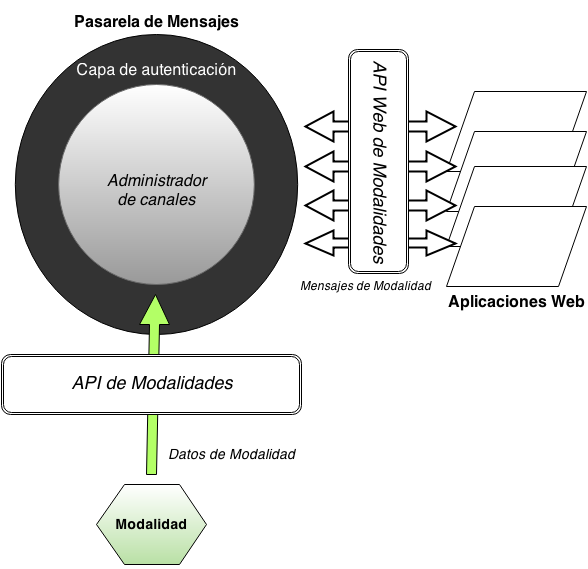
\includegraphics[scale=1,width=\textwidth]{gfx/arq_simple_es}
    \caption{Componentes de arquitectura para una aplicación web}
    \label{fig:arq_ours_single_app}
  \end{figure}
\end{center}

\subsection{Pasarela de Mensajes: Introducción} \label{sec:arq_ours_intro}
En la figura \ref{fig:arq_ours_single_app} se puede observar de manera rápida la arquitectura del sistema. En esta sección se pondrá el foco sobre el \emph{Message Gateway} o \emph{Pasarela de Mensajes}; de ahora en mas se usará PM para referirse a la misma con el fin de abreviar.
En la construcción de la PM se tuvo en cuenta un modelo de capas, con el \emph{Channels Manager} o \emph{Administrador de canales} como núcleo y único componente requerido para su funcionamiento. El resto de las capas agrega funcionalidades, de manera muy similar a la de un \emph{middleware}. Es decir, interceptan los mensajes, los utilizan como entrada para ampliar el contexto, validar el pedido o cualquier otra tarea que pueda hacerse con los datos del mensaje; luego de realizada dicha tarea, le pasan el mensaje al siguiente nivel de profundidad hasta llegar al núcleo.

El núcleo, a través de una base de datos en memoria, mantiene los canales activos de comunicación. Un canal equivale a una aplicación. Los canales pueden ser multiplexados, es decir, usando un canal, podemos fragmentarlo y generar sub-canales en caso de ser necesario. 
El núcleo, implementa un patrón similar al de \emph{Publishers/Subscribers}, entonces, de forma simple, cuando recibe un mensaje, chequea el canal por el cual debe retransmitirlo hacia todos los clientes suscritos al mismo. Como se ha mencionado antes, es valido visualizar una cardinalidad 1 a 1 entre canales y aplicaciones. 

Por otra parte, una aplicación puede tener \emph{N} clientes. Cada cliente conectado a la aplicación, es automáticamente suscrito a su correspondiente canal, a través de la API provista al navegador (usando el módulo \emph{Gyes} que veremos en el próximo capitulo). De manera similar, la modalidad, a través de la interfaz provista para las mismas se conectará al canal de aplicación que le corresponda. Ya sea una persona (desarrollador) o un equipo de trabajo multimodal, deberán tener acceso al token de acceso por aplicación. Este token podría ser accedido mediante alguna aplicación de registro a la plataforma como servicio o podría ser simplemente generado y distribuido internamente en el grupo de trabajo, si se toma la decisión de hostear de forma autónoma una instancia de la plataforma. 

De cualquier manera, se genera un puente entre modalidad y aplicaciones cliente, lo que equivale a decir que es posible intercambiar mensajes bidireccionalmente entre aplicaciones ``cliente'' y modalidades conectadas a la aplicación. Por lo que no solo los clientes se ven afectados por la señal generada por la modalidad, si no que ellos también pueden modificar, por ejemplo, la configuración de la modalidad en tiempo-real. La cual es una característica con la que muy pocos sistemas multimodales cuentan.

\marginpar{PaaS o en español, plataforma como servicio, hace referencia a una plataforma en la nube que brinda una solución que puede ser aplicada por el consumidor como una capa mas a su sistema, abstrayéndolo de diferentes cuestiones relacionadas al hardware y brindándole capacidades de escalabilidad.}
Otra capa importante pensando en la plataforma como PaaS (\emph{Platform as a Service}), y que esta provista en el sistema de forma inicial, es la de autenticación (\emph{Authentication Layer}). La forma de autenticar clientes es algo simple, pero efectiva para el caso. Se basa en una estrategia tipo ``algo que posea'' el cliente. En este caso, al registrar una aplicación web que usará esta plataforma, la misma recibirá un \emph{token}. Tanto el desarrollador de modalidad (si es que lo hay), como el desarrollador de la aplicación web, comparten este token. El sistema registra a la aplicación con un token y un canal. Cabe destacar que en este aspecto puntual, por aplicación se refiere tanto a las modalidades usadas como a los clientes web (son todos ``parte de'').

Al llegar un mensaje nuevo, tanto por parte de un cliente como de una modalidad, esta capa lo intercepta, toma el token que viene con el mensaje, y lo valida. Si es positiva, el mensaje continua a la siguiente capa, y se cachea el token para mejorar la performance en futuros mensajes. Si no es valido, el mensaje es desechado y no continua. Este proceso se describe aquí de manera rápida, porque el foco, por el momento no esta puesto en la seguridad del sistema, pero se cree que es un mecanismo que junto con otras previsiones puede garantizar autenticidad sin producir demasiado \emph{overhead} en la comunicación.

\subsection{Pasarela de Mensajes: Diseño} \label{sec:arq_ours_design}
La pasarela de mensajes \emph{Plusultra}, esta implementada usando un esquema de interacción distribuida tipo \emph{publish/subscriber}, ver figura \ref{fig:infra_pubsub}. Se decidió utilizar un esquema de comunicación basado en eventos para favorecer a los dispositivos de modalidad, los principales productores del sistema. Los dispositivos de modalidad pueden ser clasificados como reconocedores, sintetizadores o ambos. De cualquier forma, estos se comunicarán a través de eventos, \eg generando uno luego de reconocer un gesto (patrón) o recibiendo un evento que señalice la ocurrencia de una fisión, dando lugar a una posible acción de sintetizado.

% FIGURA DE PUBSUB
\begin{center}
  \begin{figure}[h]
    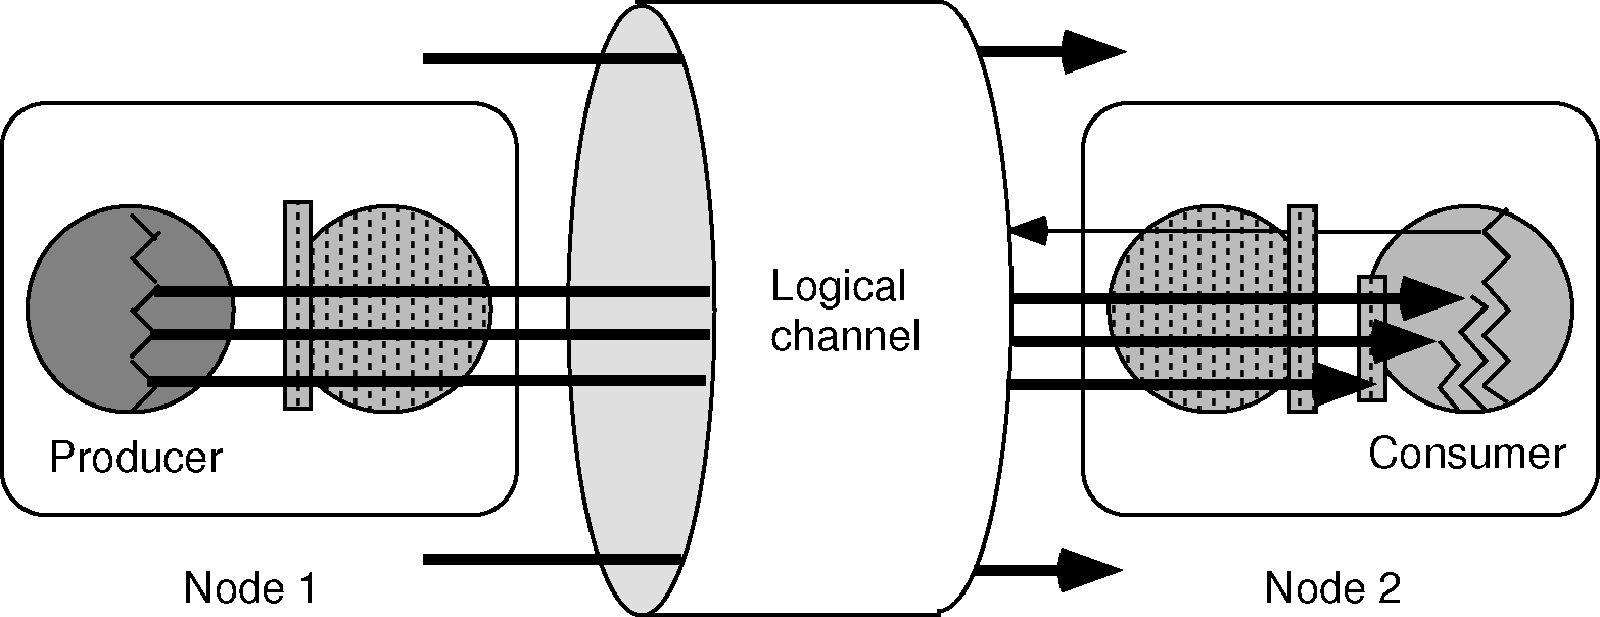
\includegraphics[scale=1,width=\textwidth]{gfx/pubsub}
    \caption{El paradigma de interacción Publishers/Subscribers, de acuerdo a \citet{Kermarrec2003}.}
    \label{fig:infra_pubsub}
  \end{figure}
\end{center}

Los eventos pueden ser mensajes en texto plano o con algún formato, como JSON en este caso. Los mismos encapsulan un protocolo de comunicación que se definirá junto al modulo cliente \emph{Gyes}, mas adelante. 

\marginpar{Redis, es un sistema open source, que permite almacenamiento y cacheo de estructuras \emph{clave-valor}. Es también conocido como un servidor para estructuras de datos. Para mas información visitar: \href{http://redis.io/}{redis.io}}
La información sobre canales y aplicaciones activas es almacenada utilizando algún sistema de base de datos en memoria, en la implementación actual se utiliza \textbf{Redis} (configurado especialmente para no persistir datos), esto permite un acceso rápido a la información de una aplicación y ayuda a perfilar a la plataforma como un sistema de intercambio de mensajes volátil, es decir, esto no es una base de datos ni una cola de mensajes. 

Cada instancia de la pasarela funciona como un modulo \emph{productor/consumidor} distribuido. Esto permite ver al sistema en general como un motor de notificación de eventos distribuido en un conjunto de procesos y servidores, compartiendo diferentes bases de datos en memoria. Esta visión se corresponde con la del sistema funcionando como un PaaS, aunque también puede correr \emph{standalone}, es decir, como una unidad de trabajo particular. Esta forma de ver al sistema corresponde con una arquitectura \emph{publishers/subscribers} centralizada, muy similar a una cola de mensajes. 

Las principales ventajas de implementar a \emph{Plusultra} como un sistema de notificación \emph{publish/subscriber} radican en tres cualidades, de acuerdo con \citet{Kermarrec2003}:
\begin{itemize}
\item \textbf{Desacoplamiento en tiempo}; las partes que interactúan, dispositivos de modalidad y aplicaciones, no necesitan estar conectadas al mismo tiempo para comunicarse. Los dispositivos de modalidad son independientes al número de clientes conectados y viceversa. La importancia radica en el momento, esto es, si se produce una señal entonces puedo captarla y hacer algo; ``si ocurrió una señal en el pasado no me interesa''.

\item \textbf{Desacoplamiento en espacio}; este desacople se produce entre aplicaciones y dispositivos de modalidad e implica que no es necesario que estos entes se conozcan entre ellos para funcionar. Las dispositivos envían señales, en forma de eventos, hacia la plataforma y continúan su trabajo. Por otra parte, los clientes, es decir las aplicaciones web, cuando detectan una nueva fusión (que pudo haberse producido) por una señal de una modalidad, pueden ejecutar un \emph{callback} asociado en ese momento. 

\item \textbf{Desacoplamiento en sincronización}; No ocurre ningún tipo de bloqueo entre dispositivos de modalidad y clientes web. Cuando una señal es reconocida y un evento es disparado, el driver del dispositivo nunca esperará por una respuesta para ``continuar''. De forma similar, cuando algo ocurre y se debe señalizar a una aplicación, este evento particular generará la ejecución de un \emph{callback} en el cliente; es decir, éste nunca se detuvo a esperar por la ocurrencia de dicho evento.

\end{itemize}

La plataforma fue diseñada teniendo en cuentas estas características. Mas aun, un sistema desarrollado teniendo en cuenta estos items tendrá facilidades al momento de escalar \citep{Kermarrec2003}.

Los desafíos o posibles inconvenientes a los que puede verse afectado un sistema de notificaciones de este tipo se encuentran en el hardware y plataforma sobre la que corran, así como también de las posibles limitaciones en la topología y protocolos de comunicación usados. Por ejemplo, el sistema puede verse beneficiado si se utiliza un protocolo de comunicación probabilístico en lugar de uno diseñado para \emph{WAN} como RMTP, que genera \emph{overhead} debido a la gran cantidad de mensajes de confirmación que ocurrirían \citep{Kermarrec2003}.
La extensión y consolidación de esta \emph{Plusultra} como PaaS queda fuera del alcance de este trabajo y sería posible analizarla solo con mas tiempo y en condiciones diferentes.

\subsection{Pasarela de Mensajes: Implementación} \label{sec:arq_ours_code}
Para implementar la pasarela se ha decidido utilizar \textbf{Node.js}. Esta tecnología, comprende a un entorno de desarrollo multi-plataforma (gracias al motor V8 en el que corre), orientado a I/O y con una arquitectura basada en eventos, lo que lo convierte en una herramienta favorable para desarrollar servicios o aplicaciones orientadas a \linebreak{\emph{networking}}, como es el caso de la plataforma aquí propuesta; donde el foco esta puesto en las comunicaciones y no en el procesamiento.
Otra ventajas de usar Node.js, es que se mantiene un mismo lenguaje para el código del proyecto: JavaScript. Haciendo mas fácil pasar de una tarea a otra. Por ejemplo cambiar de contexto, al desarrollar un modulo cliente y luego volver a la plataforma.

\section{Comparación con la Arquitectura Clásica} \label{sec:arq_others}
Se considera como \emph{arquitectura clásica} para un sistema con interacciones multimodales a la definida por \citet{dumas2009multimodal}. En dicho trabajo, los autores abstraen las características genéricas que un sistema multimodal debería poseer, definen componentes arquitectónicos fundamentales. 

% FIGURA DE COMPONENTES ARQ CLASICOS - Dumas
\begin{center}
  \begin{figure}[h]
    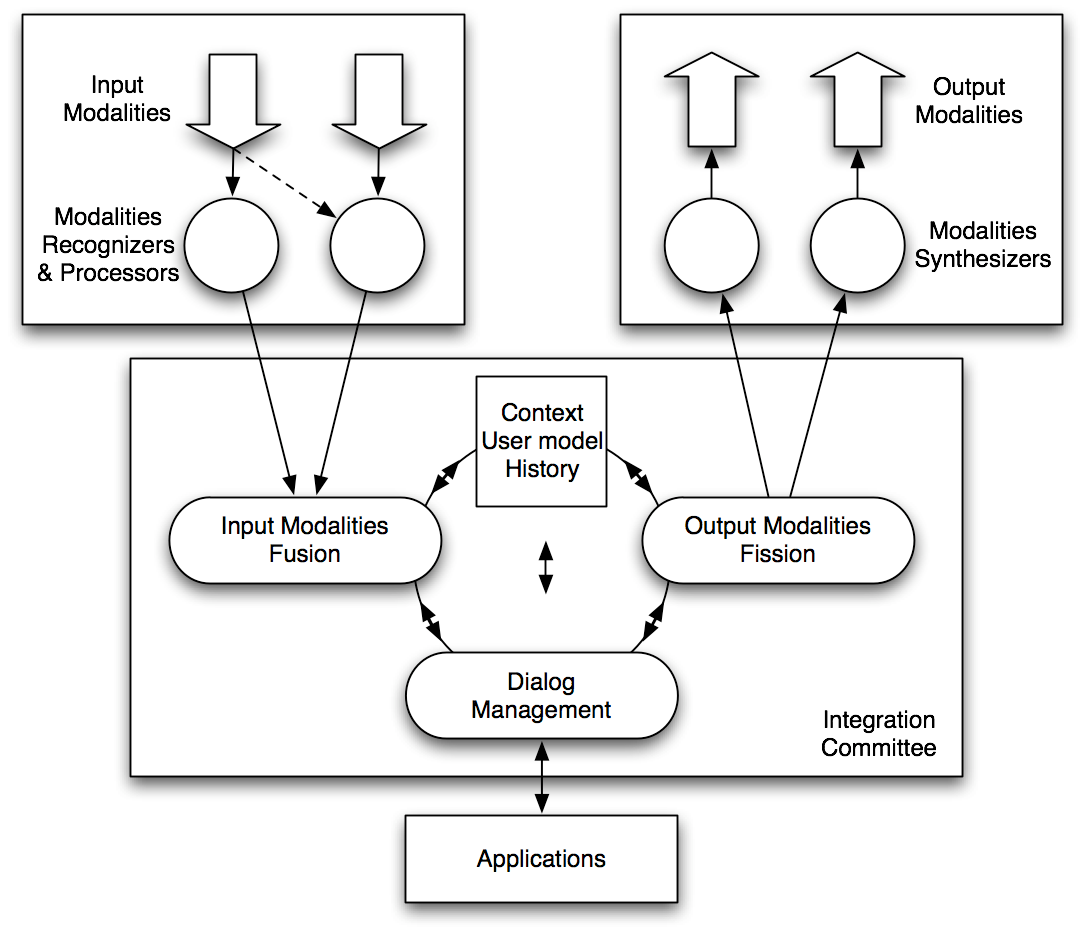
\includegraphics[scale=1,width=\textwidth]{gfx/arq_dumas}
    \caption{La arquitectura de un sistema multimodal clásico por  \citet{dumas2009multimodal}.}
    \label{fig:arq_others_dumas}
  \end{figure}
\end{center}

En la figura \ref{fig:arq_others_dumas} se pueden observar los principales componentes, el \emph{comité de integración} con sus sub-componentes y las modalidades con los correspondientes, \emph{reconocedores}, \emph{pre-procesadores} y \emph{sintetizadores} entre otros posibles filtros.

Este es un esquema claro en cuanto a la división de responsabilidades. La arquitectura propuesta en este capitulo se concentra en la forma de interconectar las modalidades, la implementación realizada del \textbf{comité de integración} será analizada en el próximo capitulo.
De acuerdo a las características antes mencionadas, la arquitectura debe ser capaz de insertarse en un ambiente distribuido. Es decir, debe ser capaz de conectar de una forma clara y efectiva modalidades (entrada y salida) con múltiples clientes de una aplicación web, en tiempo real. Para eso, como ya se ha mencionado, se utiliza un sistema de interconexión basado en eventos. Entones, re-interpretando la arquitectura clásica, el diseño de la solución propuesta se ve en la figura \ref{fig:arq_dumas_plusultra}.

% FIGURA DE COMPONENTES ARQ CLASICOS - Dumas + Plusultra
\begin{center}
  \begin{figure}[h]
    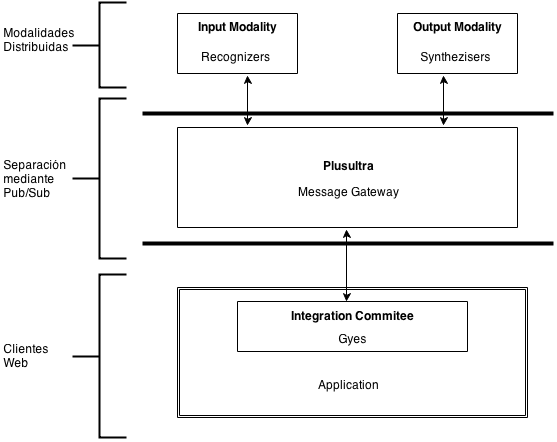
\includegraphics[scale=1,width=\textwidth]{gfx/Dumas_Plusultra}
    \caption{La arquitectura propuesta en este trabajo.}
    \label{fig:arq_dumas_plusultra}
  \end{figure}
\end{center}

La \emph{pasarela de mensajes}, se convierte en un aspecto central, que permite mantener la separación de responsabilidades original de la aplicación y a la vez adaptarse al contexto de una aplicación web.

Ese diseño brinda otra ventaja, importante si se piensa a la \emph{plataforma como servicio}, se trata de la capacidad para escalar horizontalmente, como se ha mencionado en la sección \ref{sec:arq_ours_design}. En el siguiente gráfico \ref{fig:ours_single_app_scalable_scenario} se muestra un hipotético escenario escalable. Esta es solo una configuración posible para conseguir escalabilidad, utiliza un balanceador de carga como una dependencia externa (\ie nginx); otra alternativa podría desechar la necesidad de agregar otro componente mediante el desarrollo de una nueva capa de ``middleware'' que auto-balancee la carga y distribuya a otro cliente, de los posibles instanciados por el usuario de la plataforma. Hay mas alternativas para explorar y queda abierto (escapando a los objetivos del presente trabajo), en el campo de PaaS o de servicios sobre Internet en general, elegir y probar los mejores caminos.

% FIGURA DE COMPONENTES ARQ - our, scalable
\begin{center}
  \begin{figure}[h]
    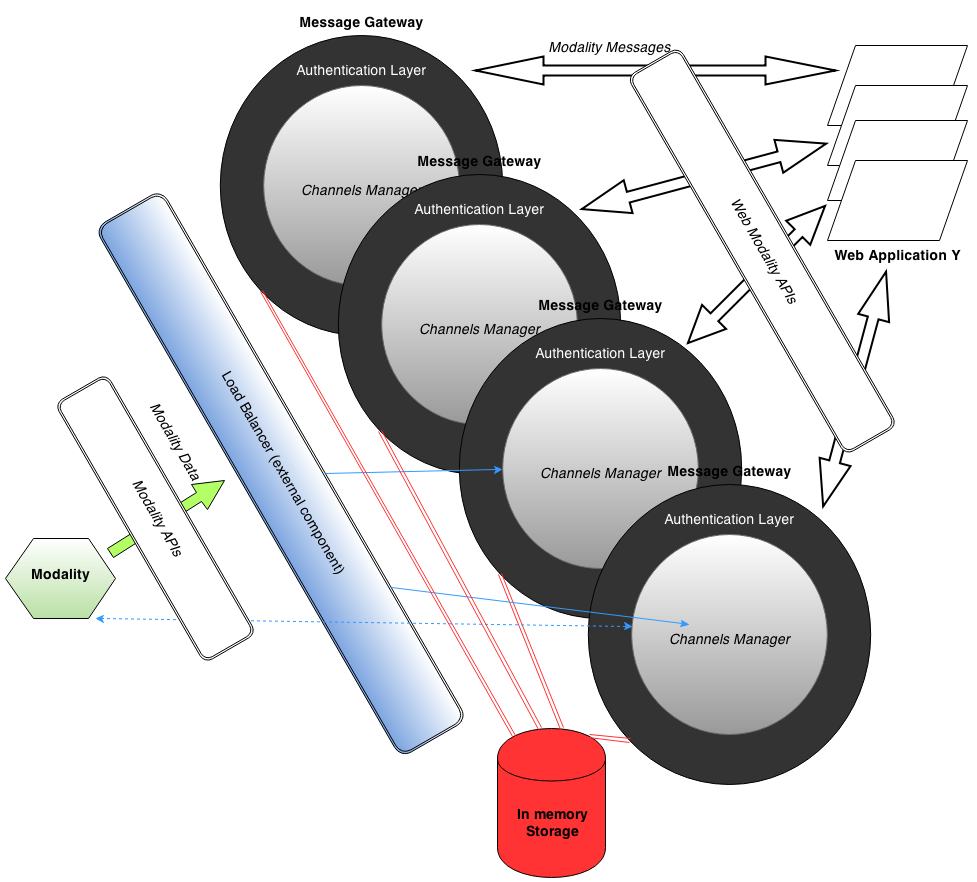
\includegraphics[scale=1,width=\textwidth]{gfx/arq_scalable}
    \caption{Componentes de arquitectura en un escenario escalable, múltiples PMs.}
    \label{fig:ours_single_app_scalable_scenario}
  \end{figure}
\end{center}


\section{Comparación con la Arquitectura Propuesta por la W3C} \label{sec:arq_others_w3c}
En \citet{w3c:mmiarch}, se propone una arquitectura similar a la denominada ``clásica''. Dentro del \emph{Runtime Framework}, donde se definen muchos aspectos técnicos y que esta delegado a quien implemente la arquitectura se define un \emph{Interaction Manager}(administrador de interacción) o IM, que debe recibir todos los eventos generados por los diferentes \emph{Modality Components}(componentes de modalidad) o MC; allí se define la interacción con el componente. Algo similar a los componentes de fisión y fusión de la arquitectura clásica, solo que aquí se encuentran distribuidos. El modulo IM es similar a la pasarela de mensajes de la estrategia propuesta. La diferencia radica, en parte, en la fuerte orientación a eventos y a trabajar como máquina de estados por parte del IM. En cambio el componente PM, en un principio, esta orientado a trabajar transmitiendo datos en ``crudo'' por parte de las modalidades y no eventos. Aunque esto puede modificarse, añadiendo algún tipo de pre-procesador de los datos generados por la modalidad. Esto depende del ingeniero de modalidad.

Las modalidades se definen usando algún tipo de lenguaje de marcado (\ie CCXML, SCXML, HTML, entre otros). Otra diferencia importante entre el sistema propuesto por la W3C y el del presente trabajo, es la API que conecta el IM con los diferentes MC. Es la sección menos flexible del documento \citet{w3c:mmiarch}. En ella se definen cuestiones tales como activación y detención de la modalidad, acciones previas a recibir un mensaje, inicio y fin de la conversación. Esta API le da fuerza al modelo de máquina de estados. 

En este trabajo no se considera un modelo de maquina de estado porque en un principio se busca favorecer al máximo, o lo que es lo mismo, minimizar cualquier tipo de obstactulo en la transmisión de datos ``crudos''. Por otra parte, la estrategia aquí presentada, mueve los componentes de fisión y fusión a los clientes y le entrega dicha responsabilidad al desarrollador de la aplicación para que fusione con libertad el contexto de la aplicación que esta desarrollando con las modalidades disponibles. Se cree que de esta manera se puede explotar el uso de las modalidades.

En el gráfico \ref{fig:arq_others_w3c} se muestra la arquitectura propuesta por la W3C antes mencionada.
% FIGURA DE COMPONENTES ARQ - others, w3c
\begin{center}
  \begin{figure}[h!]
    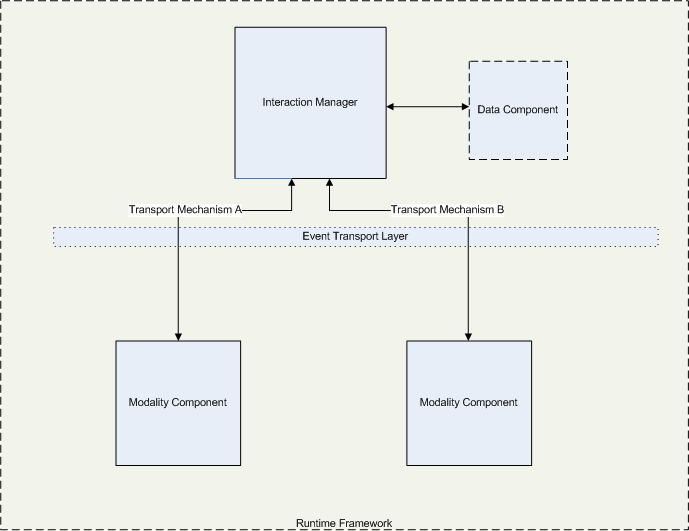
\includegraphics[scale=1,width=\textwidth]{gfx/w3c_RevisedArchDiagram}
    \caption{Arquitectura de la W3C en tiempo de ejecución}
    \label{fig:arq_others_w3c}
  \end{figure}
\end{center}
\large

\hfill
\vfill

\section{Resumen del Capítulo} \label{sec:infra_summary}
En este capítulo se ha mostrado la estrategia elegida en la creación de la arquitectura necesaria para poder expandir las capacidades de las aplicaciones web actuales con el uso de nuevas modalidades. Se han detallado características particulares al ambiente de las aplicaciones web y que han influido en las decisiones tomadas para desarrollar dicha arquitectura. A su vez, se ha comparado el trabajo realizado con otras soluciones conocidas, como son el modelo presentado por \citet{dumas2009multimodal} y el trabajo del grupo de MMI \citet{w3c:mmiarch}

Mas adelante, se completara la arquitectura, definiendo la implementación elegida para el ``núcleo'' de la misma, como son los componentes de \emph{fusión} y \emph{fisión}; con el fin de mantener la claridad se ha decidido analizarlos por separado.


%############################################################################